%! TEX root = ../thesis.tex
\documentclass[../thesis]{subfiles}
\graphicspath{{\subfix{../figures/}}}

\begin{document}
\chapter{Concepts}\label{ch:concepts}

%\lettrine[lines=3]{\textcolor{Maroon}{B}}{efore} tackling the implementation, we need to take a closer look at the concepts central to this thesis, so that we can form a concrete idea of which parts of \gls{lsp} are well-suited to being integrated into \glspl{city}.
\lettrine[lines=3]{\textcolor{Maroon}{O}}{utlining} the central concepts behind this thesis is a crucial first step before tackling the implementation, so that we can form a concrete idea of which parts of \gls{lsp} are well-suited to being integrated into \glspl{city}.
Thus, we will examine the concept of \glspl{city}, where we will use \SEE{} as a concrete implementation (which we do in \cref{sec:see}), as well as the \glsentrylong{lsp} (which we do in \cref{sec:lsp}).
For the former, we will go over some of the existing literature regarding \glspl{city} (as this is more of an academic topic than \gls{lsp}) and describe the essentials that we need to work with in the implementation, such as the project graph.
As for the latter, we will go over the available \glspl{capability} and take a look at both existing \glspl{ls} and \glspl{lc} to get an idea of what the \glsentrylong{lsp} offers and how it is most commonly used.
For both topics, we will focus on the parts relevant to the implementation and evaluation---for example, we will only explore those \glspl{capability} in detail that actually end up being used in this thesis.

\section{SEE}\label{sec:see}

As explained in \cref{subsec:see}, \SEE{} is an interactive software visualization tool using the \gls{city} metaphor in 3D, with the aim to make it easier to work with large software projects on an architectural level.
To name a few example scenarios in which using code cities could be useful, compared to using traditional \glspl{ide}:
\begin{itemize}
	\item Senior developers may use it in its "multiplayer" mode to explain the structure of their software to newcomers
	\item Project planners could visualize \glspl{smell} to find candidates for refactoring~\cite{galperin2021}
	\item Software architects can find violations of the planned architecture using \SEE{}'s \gls{reflexion}
\end{itemize}

\SEE{} is an open-source project, currently hosted at GitHub\footnote{\web{https://github.com/uni-bremen-agst/SEE}{2024-09-18} (but note that, to clone this repository, you additionally need access to the Git LFS counterpart hosted at the University of Bremen's GitLab, as this is where paid plugins for \SEE{} are hosted.)}.
It is a research project at the University of Bremen, where it has been in development since 2017~\cite{ganser2017}, and where it is frequently offered as a bachelor or master project for the students.
While it was at first a project for the \emph{Unreal Engine}, the game engine has been switched to \emph{Unity} relatively early, mainly because its editor eased development due to the ability to reload the \gls*{ui} without having to restart the whole engine.

After going over the basics of how \SEE{} works, I will give an explanation and formalization of the project graph---as this is the central component in the \gls{lsp}-based \gls{city}-generation algorithm---followed by a brief overview over other features that are relevant for this thesis.

\subsection{Basics}
As mentioned before, when analyzing a software project in \SEE{}, its source code structure is reflected in the rendered buildings, where connections between the components, such as references, are displayed using edges rendered as splines (this will be elaborated in \cref{subsec:graph}), as can be seen in \cref{fig:edges}, for example.
Metrics of the project, such as the McCabe complexity~\cite{mccabe}, can then be mapped onto visual properties of this rendering, such as its color, width, or height.

So far, the kind of visualization described here would still be possible in two dimensions, but adding a third dimension gives us the benefit of having another axis to map metrics onto, as well as making it a more natural environment for humans to interact with.
By giving users the ability to walk, move the camera around, and so on, as is possible in many video games, the code city can be navigated in a richer and more intuitive manner than if it were just a simple 2D image.
This also makes it possible to offer \SEE{} as a virtual reality application.
Virtual reality gives users an even more immersive and natural way of interacting with the environment, leading to improved spatial memory of the city~\cite[\eg,][]{tavanti2001}.
It also makes it a more fitting environment for multiple people.
Each player can have their own avatar placed in the scene, interacting with one another and the city, communicating via voice chat.

As an interactive game-like project such as this comes across more clearly in a video than in mere text and disconnected snapshots, readers can take a look at this introductory video for an overview of \SEE{}: \web{https://www.youtube.com/watch?v=fYMRpmuk7To}{2025-01-06}.

\subsection{Project Graph}\label{subsec:graph}

We will now take a look at the graph representing the source structure of the analyzed software projects in \SEE{}.
One of the main goals of this thesis is generating such a graph using \gls{lsp}, as opposed to the currently available methods of generating this graph, which require access to the proprietary Axivion Suite to create the \gls{gxl} files used in \SEE{}.

These graphs can be formalized as $G = (V, E, a, s, t, \ell)$, with:
\begin{itemize}
	\item $V$ being a set of nodes and $E$ being a set of edges.
	\item $a: (V \times \mathcal{A}_K) \rightharpoonup \mathcal{A}_V$ associating nodes and an attribute name $(\in \mathcal{A}_{K})$ with a value $(\in \mathcal{A}_{V})$. Note that this is a partial function.
	\item $s: E \rightarrow V$ denoting the source node of an edge.
	\item $t: E \rightarrow V$ denoting the target node of an edge.
	\item $\ell: E \rightarrow \Sigma$ providing a label for an edge over some alphabet $\Sigma$.
	      Also, $\tt{partOf} \in \Sigma$ such that the subgraph $(V, \{e \in E \mid \ell(e) = \tt{partOf}\}, a, s, t, \ell)$ is a \gls{polytree}.
\end{itemize}

Explained in natural language:
The graph's nodes ($V$) can be connected by directed edges ($E$)---these are not necessarily unique for each possible tuple of nodes, meaning that there can be more than one edge between the same two nodes.
A node represents a component in the source code (\eg, a class), while edges represent relationships between them (\eg, inheritance).
This is an attributed graph.
Specifically, each node can have multiple attributes (distinguished by attribute keys), while each edge always has one label that denotes the type of its relationship.
The label \tt{partOf} additionally has a special meaning: edges with this type induce the hierarchy of the source code (\eg, classes contained in files).
Hence, if we look at the graph that removes all edges except for those with label \tt{partOf}, and we make these edges undirected, we get a tree.

To illustrate, a few examples of attributes are:
\begin{itemize}
	\item \tt{Source.Path}: the path to the file the element is contained in.
	\item \tt{Source.Name}: the name of the element within the source code.
	\item \tt{Type}: the type of the element (\eg{}, "method").
\end{itemize}

Another attribute that is also relevant for \gls{lsp} is the \tt{Source.\allowbreak\Gls*{range}}, which is often used in the upcoming \cref{sec:lsp,ch:implementation}.
It describes a contiguous portion of source code.
We formally define the domain of ranges $\mathcal{R}$ as the Cartesian square of positions $\mathcal{P}^2$, whereas the domain of positions $\mathcal{P}$ is defined as the Cartesian square of natural numbers (including zero), that is, $\mathcal{P} = \mathbb{N}^2_0$.
Hence, as a whole, $\mathcal{R} = \mathcal{P}^2 = \mathbb{N}^4_0$.
Semantically, a position $(l, c) \in \mathcal{P}$ describes a zero-indexed line $l$ and a zero-indexed character offset $c$, relative to the beginning of the line.
A range $(b, e) \in \mathcal{R}$ can be understood as a beginning position $b$ (inclusive) and an ending position $e$ (exclusive).
We will also occasionally "decompose" those positions and refer to a range $r$ in decomposed form as $r = \left(b_l^r, b_c^r, e_l^r, e_c^r\right)$.
For example, the interval of lines that the range $r$ (partially or completely) covers is then given by $\left[b_l^r, e_l^r\right)$.

I should note that the model presented here is a simplification of \SEE{}'s actual data model for source code graphs.
For example, in reality, edges can have multiple attributes, there can be multiple edge types other than \tt{partOf} that have the \gls{polytree} property, and so on.
This is just what is needed to understand the \gls{lsp}-based city generation algorithm presented in \cref{sec:generate}.

\subsection{Other Relevant Features}\label{subsec:seeother}

Apart from the project graph, there are a few other features of \SEE{} we need to go over, as they become relevant when integrating \gls{lsp} into \glspl{city} (in \cref{sec:intocity}) and \glspl{window} (in \cref{sec:intowindow}).

% Which are:
\paragraph{Context Menu}

\begin{figure}[htbp]
	\begin{center}
		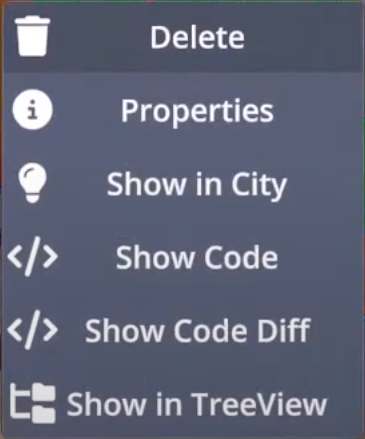
\includegraphics[width=0.3\textwidth]{OldContextMenu}
	\end{center}
	\caption{A screenshot of \SEE{}'s context menu before the changes in \cref{ch:implementation}.}\label{fig:oldcontext}
\end{figure}

When right-clicking any node or edge, a menu opens with several context-dependent options, shown in \cref{fig:oldcontext}.
These include the option to delete the element, to highlight it within the \gls{city}, to open its corresponding \gls{window}, and others.
We will expand this menu with \gls{lsp}-specific actions in the course of \cref{sec:intocity}.

\paragraph{City Editor}

\begin{figure}[htbp]
	\begin{center}
		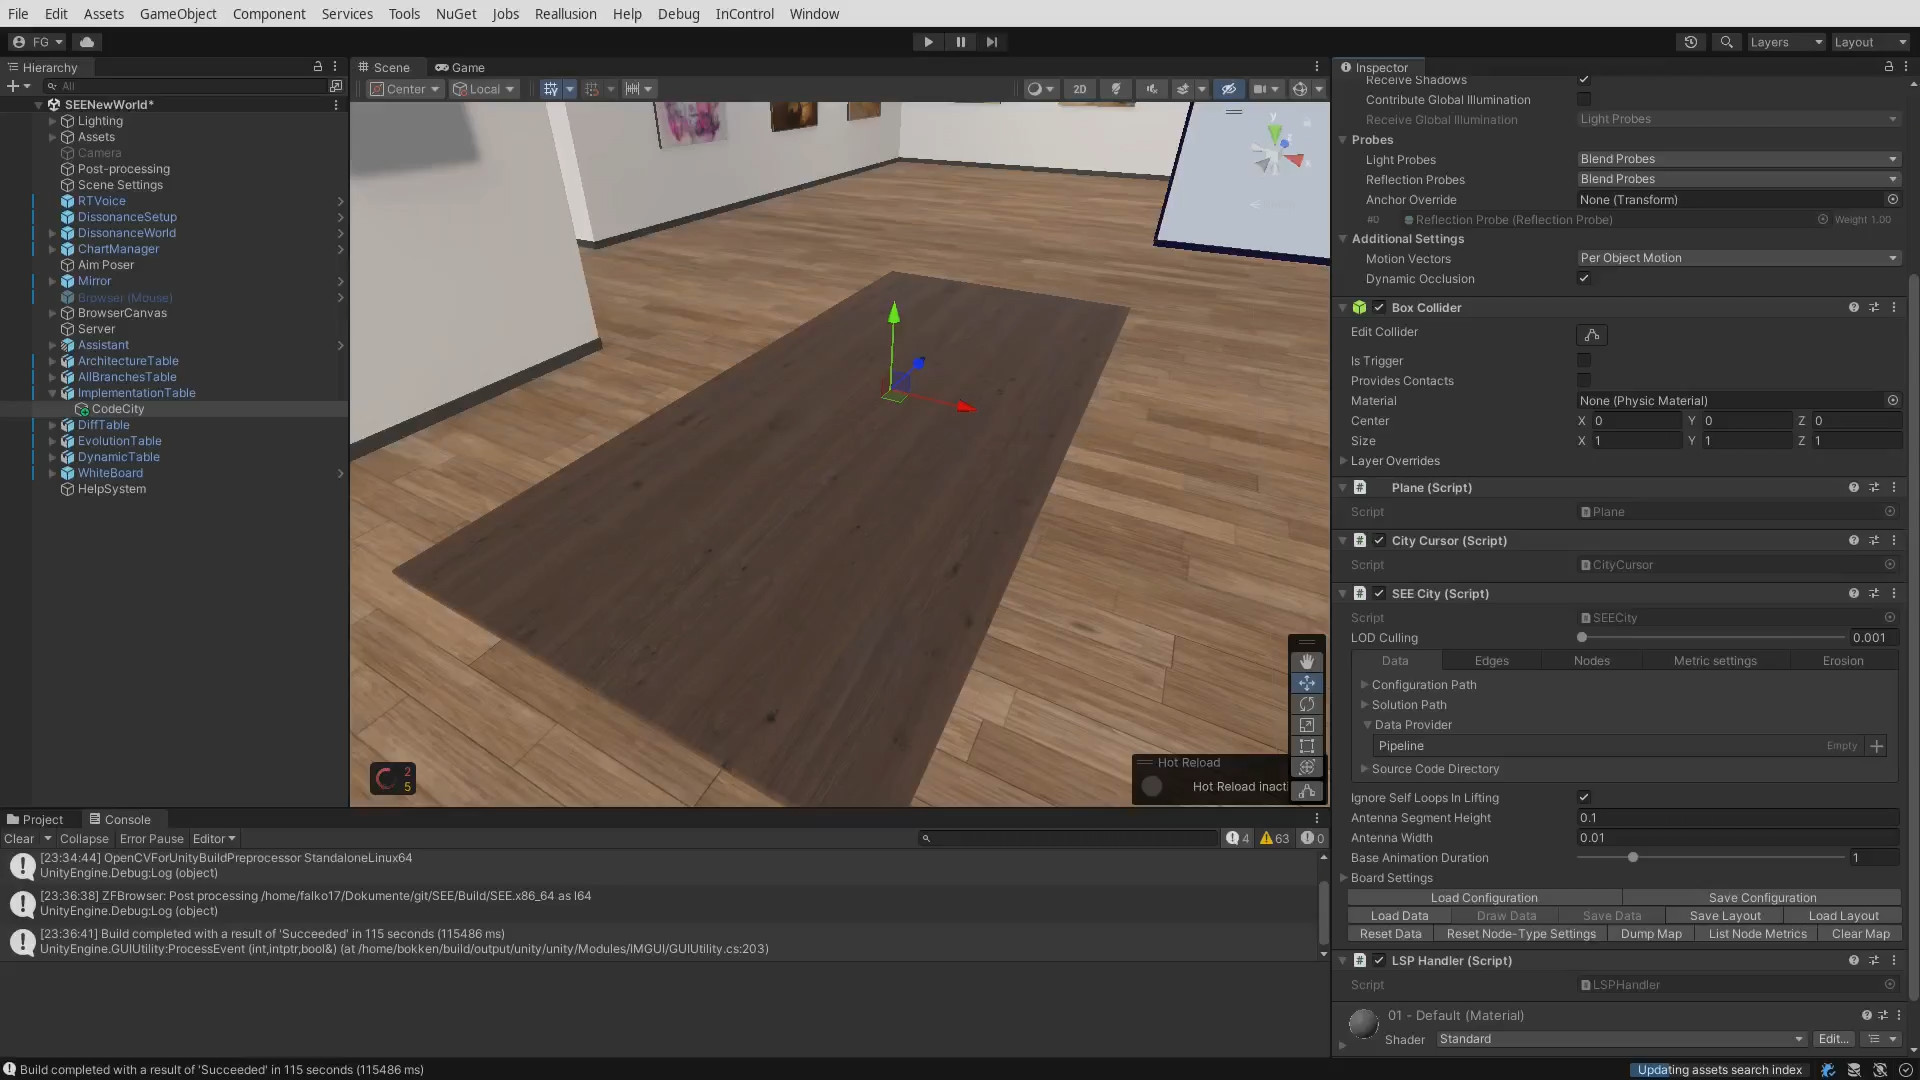
\includegraphics[width=\textwidth]{UnityEditor}
	\end{center}
	\caption{The \gls*{editor} with a scene in \SEE{} opened.}\label{fig:editor}
\end{figure}

To actually generate a \gls{city}---assuming one has a \gls{gxl} file for this purpose---a customized \gls{ui} component within the \gls{editor} exists in \SEE{}.
Here, a variety of options can be configured, such as the layout of the city, the mapping of metrics to visual attributes, or the \glspl*{provider}, which create a project graph based on optional input parameters (such as the aforementioned \gls{gxl} file).

\Cref{fig:editor} shows what the \gls{editor} looks like in \SEE{}:
On the left are the objects of the scene, the middle shows a preview, the bottom left displays log messages, and finally, the components (including the city editor component) can be seen on the bottom right.
After implementing the city-generation algorithm for \gls{lsp}, a new \gls{provider} with its own \gls{editor} \gls{ui} shall be implemented as well.

\paragraph{Code Windows}
As explained in \cref{sec:goals}, there is also the option of opening \glspl{window} to view the source code of a component, an example of which is shown in \cref{fig:window}.
Currently, these windows do little more than lexer-based syntax highlighting, so a goal is to include more \gls{ide}-like behavior by using functionality offered by \gls{lsp}.

\paragraph{Erosion icons}

\begin{figure}[htbp]
	\begin{center}
		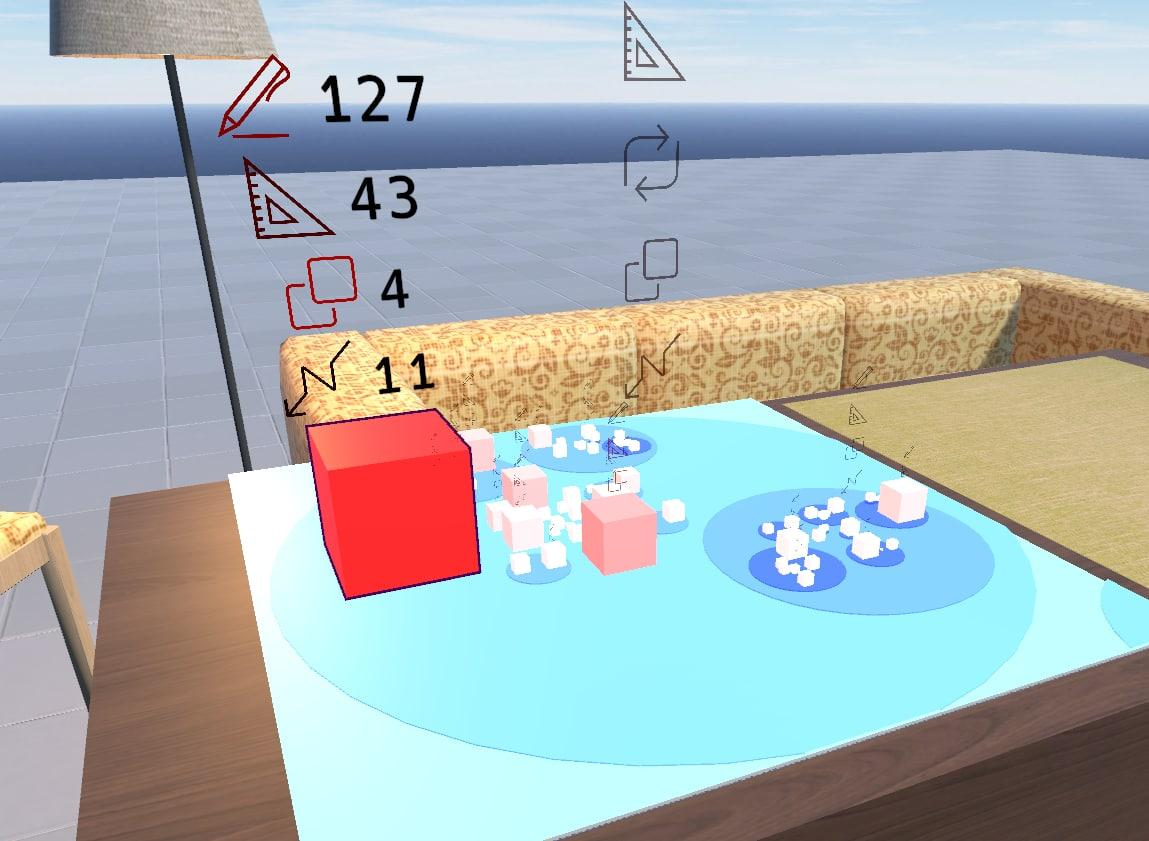
\includegraphics[width=0.9\textwidth]{ErosionIcons}
	\end{center}
	\caption{An example of \glspl{smell} visualized as erosion icons in \SEE{}.}\label{fig:erosion}
\end{figure}

Following my bachelor's thesis~\cite{galperin2021}, \SEE{} offers the possibility to indicate the number of \glspl{smell} per component using the so-called \emph{erosion icons}.
These are essentially small icons that can be put above each node, as shown in \cref{fig:erosion}.
The size and color of these erosion icons can then indicate the quantity of \glspl{smell} for that given node.
A controlled experiment has suggested that this gives developers a quicker, more intuitive overview over the distribution of \glspl{smell} within a project, compared to traditional (\ie, tabular) ways of displaying this information~\cite{galperin2022}.
While \gls{lsp} does not offer a standardized way of offering \gls{smell} information, we can use its diagnostics capability (see \cref{subsec:capabilities}) for the same purpose.

\section{Language Server Protocol}\label{sec:lsp}
The very basic concepts behing \gls{lsp} have already been explained in \cref{subsec:lsp}.
The protocol aims to make it easier for \glspl{ide} to support more programming languages---specifically, to support language-specific \glspl{capability}, which we will go over in \cref{subsec:capabilities}.
It was originally developed for Microsoft's editor \gls{vscode} and was later converted into an open-source specification\footnote{
	Available at \web{https://github.com/microsoft/language-server-protocol}{2024-10-05}.
} (though there are still \gls{vscode}-specific extensions to \gls{lsp} that are not in the official specification today).
\gls{lsp} has found widespread use:
An overview page by Microsoft lists at least 269 \glspl{ls}\footnote{\web{https://microsoft.github.io/language-server-protocol/implementors/servers/}{2024-10-05}} (\ie, servers offering support for some programming language) and 61 \glspl{lc}\footnote{\web{https://microsoft.github.io/language-server-protocol/implementors/tools/}{2024-10-05}} (\ie, \glspl{ide} or development tools).
The current (as of \today{}) version of the protocol is 3.17, with version 3.18 being under active development.

\subsection{Basics}\label{subsec:lspbasics}
Messages in the Language Server Protocol are built using \gls{jrpc}, which uses JSON to encode both requests (consisting of a method name and parameters) and responses (consisting of either a result object or an error object) for procedure calls.
Requests include an ID that a response by the server can then reference to match it up with the request it is a reply to.
There also so-called \emph{notifications}, which are in essence requests without an ID, intended to send a message server that does not warrant a response~\cite{jsonrpc,json}.
In \gls{lsp}, any message sent between the \gls{lc} and \gls{ls} consist of a header---describing the length and type of the content---followed by the content, which is always a \gls{jrpc} payload.
While the specification does not mandate it, it lists some recommended communication channels on which the protocol messages can be sent, those being \tt{stdio} (using standard input/output), \tt{pipe} (using Windows's pipes), \tt{socket} (using a socket), and \tt{node-ipc} (IPC communication over Node.js\footnote{\web{https://nodejs.org}{2024-10-05}}).

\begin{codebox}{TypeScript}{lst:lspex}{Example specification of request and response objects for the Hover {capability}.}
interface HoverParams {
  textDocument: string; /** The text document's URI in string form */
  position: { line: uinteger; character: uinteger; };
}

interface HoverResult {
  value: string;
}
\end{codebox}\label{lst:lspex}

The specification lists all available types for requests and responses as TypeScript interfaces.
A sample type definition for the hovering \gls{capability}, taken from the documentation, can be seen in \cref{lst:lspex}.
From this example, we can also see that locations within documents\footnote{
	These documents must always be textual---there is no support for binary files.
} are described by a \gls*{uri} representing the document along with a \gls{range} (which we have formalized in \cref{subsec:graph}).
The corresponding method name for this example is \tt{textDocument/hover}.

The first request from the \gls{lc} to the \gls{ls} always has to be the \tt{initialize} request, including the so-called client \glspl{capability}.
These specify the \glspl{capability} that the \gls{lc} supports.
The response from the server will be a response object that includes the analogous server \glspl{capability}.
The \gls{capability} information being sent during this initial handshake is not just a pure list of the names of the corresponding procedure names, but also includes additional details on exactly which parts are supported (or, \eg, which encodings are used), specific to each \gls{capability}.
Afterwards, both parties will then restrict their usage of \gls{lsp} to the subset of \glspl{capability} that both the client and server support.

The end of an \gls{lsp} session is marked by the \gls{lc} sending the \gls{ls} a shutdown request.
After the server confirms the success of the shutdown with a corresponding response, the client should send an exit notification that finally asks the server to quit their process.

For long-running operations, the specification also supports reporting progress on ongoing requests, and cancelling them.
The progress reports not only allow indicating the status of the request to the user (\eg, by displaying it in the \gls{lc}'s \gls{ui}), but also allows the server to return partial results to stream responses (\eg, showing the first few references to a variable while the rest are still loading).

The \gls{lc} should also notify the \gls{ls} whenever a document is opened or closed---that way, the server can, for example, start tracking diagnostics in the background as soon as a certain file is opened.
There are also notifications related to modifications to the document that the \gls{lc} should send, but these are irrelevant for us because modifying source code is out-of-scope for the \gls{lsp} integration planned in this thesis.

Apart from describing fundamentals of the protocol like the above, the biggest part of the protocol's specification are the \emph{\glspl{capability}}, that is, the \gls{jrpc} method names and types of the parameters and response objects for each feature that either the \gls{lc} or \gls{ls} can use~\cite{lsp}.

\subsection{Planned Capabilities}\label{subsec:capabilities}
The \glspl{capability} I will make use of in \SEE{} can roughly be grouped into the three categories \emph{Navigation}, \emph{Information}, and \emph{Structure}.
We will take a detailed look at each relevant \gls{capability} below, along with how exactly they will be integrated into \glspl{city}.
This level of detail is justified in the fact that the integration of the \glspl{capability} is the main focus of this whole thesis.
Note that not all \glspl{ls} support all \glspl{capability}---for example, for a language without a hierarchic type system, the \gls{capability} \emph{type hierarchy} cannot really be sensibly implemented.

\paragraph{Navigation}
This is the category containing the most \glspl{capability} that we can use for this thesis, since there are a lot of ways to navigate from one element within the source code to another.
All of these take as input the position in a document, and return any number of locations, where the locations can contain a name, a file, and a \gls{range} within the file.

All such available \glspl{capability} should appear in the context menu of \SEE{}, either upon right-clicking a node, or right-clicking a code element in a \gls{window}.
Selecting one of these navigation options from the menu should open a menu from which the user can select a single result.
If there is only one result to begin with, this step should be skipped.
Once a single result has been selected:
If the request originates from a \gls{window}, the result should be opened and highlighted in that window.
If the request instead originates from a \gls{city}, the node belonging to that result should be highlighted (\eg, by glowing and having a line pointed to it).

The other important part in \SEE{} where this should be used is when building a city (\ie, when creating the project graph), as these \glspl{capability} provides us with the information we need to create (non-hierarchic) edges.
Thus, we can create an edge $e$ for each available navigation relation between two nodes, where $\ell(e)$ becomes the type of \gls{capability} that was used.
This is not as trivial as it sounds, since the \glspl{range} these \glspl{capability} return do not necessarily exactly match the actual \glspl{range} of the referenced nodes, so we need to implement some kind of matching algorithm (which we will do in \cref{subsec:kd}).

The following navigation \glspl{capability} are available:
\begin{itemize}
	\item \textbf{Call hierarchy}: Returns the incoming/outgoing calls for the symbol at the given location.
	      Since incoming calls are already covered by the references \gls{capability}, the context menu will only contain an option for showing outgoing calls.
	\item \textbf{Go to declaration}: Returns the declaration location for the symbol at the given location.
	\item \textbf{Go to definition}: Returns the definition location for the symbol at the given location.
	      \begin{itemize}
		      \item For this \gls{capability}, another feature common in \glspl{ide} should be implemented in \SEE{}'s \glspl{window}:
		            Holding \keystroke{Ctrl}, then clicking on a symbol, directly jumps to the definition of that symbol (or opens the corresponding selection menu, if there is more than one result).
	      \end{itemize}
	\item \textbf{Go to implementation}: Returns the definition location for the symbol at the given location.
	\item \textbf{Go to type definition}: Returns the location of the type definition for the symbol at the given location.
	\item \textbf{References}: Returns the location of the references to the symbol at the given location.
	\item \textbf{Type hierarchy}: Returns the sub/supertypes for the symbol at the given location.
	      Since subtypes are already covered by the references \gls{capability}, the context menu will only contain an option for showing supertypes.
\end{itemize}

\paragraph{Information}
Using these \glspl{capability}, the user can get information about either the project as a whole, or certain components of it.
I have grouped the following \glspl{capability} into this category:
\begin{itemize}
	\item \textbf{Diagnostics}: Returns diagnostics for a given file (\eg, warnings or errors).
	      These will be integrated in exactly the same way as the Axivion Suite's \glspl{smell} in my bachelor's thesis were~\cite{galperin2021}, that is:
	      \begin{itemize}
		      \item In \glspl{city}, we will display erosion icons above affected nodes (see \cref{subsec:seeother}).
		      \item In \glspl{window}, the corresponding parts of the source code should be highlighted, while hovering over the highlighted parts should reveal the diagnostic's message and details.
	      \end{itemize}
	      Note that, instead of this being a proper request followed by a server response, this is only the case for the \emph{pull diagnostics} \gls{capability}, which has only been added in the most recent version 3.17.
	      The far more commonly used version is the \emph{push diagnostics} \gls{capability}, where the \gls{ls} sends out diagnostics for the currently opened files at its own discretion, as notifications (see \cref{subsec:lspbasics})---this makes it difficult to collect this information during city construction, a topic we will explore in \cref{sec:generate}.
	\item \textbf{Hover}: Returns hover information for a given location.
	      The specification does not specify what exactly this "hover text" should be~\cite{lsp}, but most implementations of \glspl{ls} display the documentation of the hovered element, or the signature if it's a method, or other helpful associated details.
	      We can simply implement this part of the specification as intended:
	      If the user hovers above an element in a \gls{window}, or a node in a \gls{city}, we should reveal the hover information in some kind of box near the mouse cursor, hiding it again once the cursor is moved away.
	\item \textbf{\Glspl*{token}}: Returns \glspl*{token} for the given file, which are intended for syntax highlighting.
	      Similar to normal (\eg, lexer-based) syntax highlighting, requesting \glspl{token} for a document yields a list of tokens containing their positions and a type, where the type can be one that is specified in the protocol (\eg, \tt{enum}) or one that was previously announced as supported in the client \glspl{capability}.
	      \glspl{ide} can then render each token type in a different color.
	      An interesting addition to usual syntax highlighting is that each token can also be affected by any number of \emph{token modifiers}, where each modifier may add an additional rendering effect on top of the type-based color.
	      For example, tokens with the \tt{static} modifier might be rendered in \textit{italics}, while ones with the \tt{deprecated} modifier could be rendered in \st{strikethrough}.

	      \SEE{} currently uses \textsc{Antlr}\footnote{\web{https://www.antlr.org}{2024-06-10}}-based syntax highlighting, where we need to manually group each parser's token into some categories to determine colors.
	      The added value of the \glspl{token} \gls{capability} here would be ease of use (\ie, no need to manually configure each \gls{ls}) on the one hand, and support for token modifiers (\ie, "extended" syntax highlighting) on the other hand.
\end{itemize}


\paragraph{Structure}
This category actually only comprises a single \gls{capability}---one that we can use to build the hierarchy of the \gls{city}'s project graph (outlined in \cref{subsec:graph}), because it gives us information about the structure of the project.
The \gls{capability} I am talking about here is the \emph{document symbols} \gls{capability}.
Given a document, it will return all symbols present within that file, along with some additional information for each symbol, such as its type or \gls{range}.

There are actually two different possible kinds of symbols that this \gls{capability} may return:
\begin{enumerate}
	\item an array of \tt{SymbolInformation}, which is \textquote[\cite{lsp}]{a flat list of all symbols} that should not be used to infer a hierarchy.
	      Because of this limitation, if a \gls{ls} is only able to return symbols of this data type, we cannot use it to build \glspl{city}.
	      This is an older data type, and instead modern \glspl{ls} should rather return
	\item an array of \tt{DocumentSymbol}.
	      This contains a field \tt{children}, which stores \tt{DocumentSymbol}s that are contained in this one.
	      Using this property, we can establish a hierarchy and build a \gls{city} by recursively enumerating all \tt{DocumentSymbol}s and their children for each file, then querying for all relevant information by using the other \glspl{capability} outlined before.
\end{enumerate}

\subsection{Unplanned Capabilities}\label{subsec:unplanned}
There are a number of \glspl{capability} that I will not implement into \SEE{}.
These can be grouped into roughly three categories, based on the reasoning behind them being unused:
The first concerns those \glspl{capability} that relate to editing only and provide no features related to simply viewing code---as explained in \cref{sec:goals}, editing code is not part of the goals here and requires additional large-scale preparatory changes to \SEE{}.
The second concerns the complex \glspl{capability}, that is, ones whose implementation would take a lot of time and effort and thus go beyond the scope of this master's thesis.
The third concerns the niche \glspl{capability} that provide only a very marginal benefit, or do so only in rare situations.
For these, I also have not deemed the effort worth it to implement them, at least not as part of this thesis.

I will quickly list the contents of all these groups here.

\paragraph{Editing \glspl{capability}}
\begin{itemize}
	\item \textbf{Code Actions}: Allows the programmer to apply refactoring actions to the code, such as importing a referenced library.
	\item \textbf{Completion}: Computes autocomplete items while the user is typing, and applies them when chosen.
	\item \textbf{Formatting}: Applies automatic formatting to a file, or range, of code.
	\item \textbf{Rename}: Executes a project-wide rename of a symbol, which also renames all references to that symbol.
	\item \textbf{Linked Editing Range}: Returns a list of \glspl{range} that will be edited upon executing a rename of a symbol, with the purpose of highlighting those ranges during the rename.
	\item \textbf{Signature Help}: Returns signature information at the given cursor information.
	      This may seem relevant for our purposes, but it is actually intended to be shown while editing (\eg, highlighting the active parameter as one types), and its information is given by the hover \gls{capability} anyway in almost all cases.
\end{itemize}
\paragraph{Niche \glspl{capability}}
\begin{itemize}
	\item \textbf{Document Color}: Lists all color references in the code (\eg, symbolic references like \tt{Colors.red}) along with their color value in the RGB format.
	\item \textbf{Color Presentation}: Allows users to modify color references in the code by using a color picker.
	\item \textbf{Document Link}: Returns the location of links in the document.
	\item \textbf{Code Lens:} Returns commands that can be shown next to source code, such as the number of implementers of an abstract method.
	\item \textbf{Monikers:} This is a description of what symbols a project imports and which ones it exports, and is intended to make relations between multiple projects possible.
	      As \gls{lsp} usually only deals with a single project at a time, this is more useful in the \gls{lsif}, whose specification it also originates from~\cite{lsif}.
\end{itemize}
\paragraph{Complex \glspl{capability}}
\begin{itemize}
	\item \textbf{Folding Range}: Returns \glspl{range} that can be collapsed in the code viewer.
	      For example, the contents of a function could be collapsed, leaving only its signature visible.
	      Due to the way \glspl{window} are implemented in \SEE{}, this would increase the complexity of the implementation quite a bit.
	\item \textbf{Inline Value}: In debugging contexts, this supplies the contents of a variable with the purpose of displaying them inline in the \gls{lc}, next to the variable itself.
	      It uses the \gls{dap}~\cite{dap}, which has previously already been integrated into \SEE{}~\cite{rohlfing2024}, but it would take a lot of refactoring work to make the two implementations compatible with each other.
	\item \textbf{Inlay Hint}: Returns textual hints that can be rendered within the source code.
	      An example would be parameter names that are intended to be shown at the call site, such as in the screenshot in \cref{fig:inlay}.
	\item \textbf{Notebook-related \glspl{capability}}: These are intended for interactive notebook systems such as Jupyter\footnote{See \web{https://jupyter.org/}{2024-10-03}}, which \SEE{} does not currently support.
\end{itemize}

\begin{figure}
	\begin{center}
		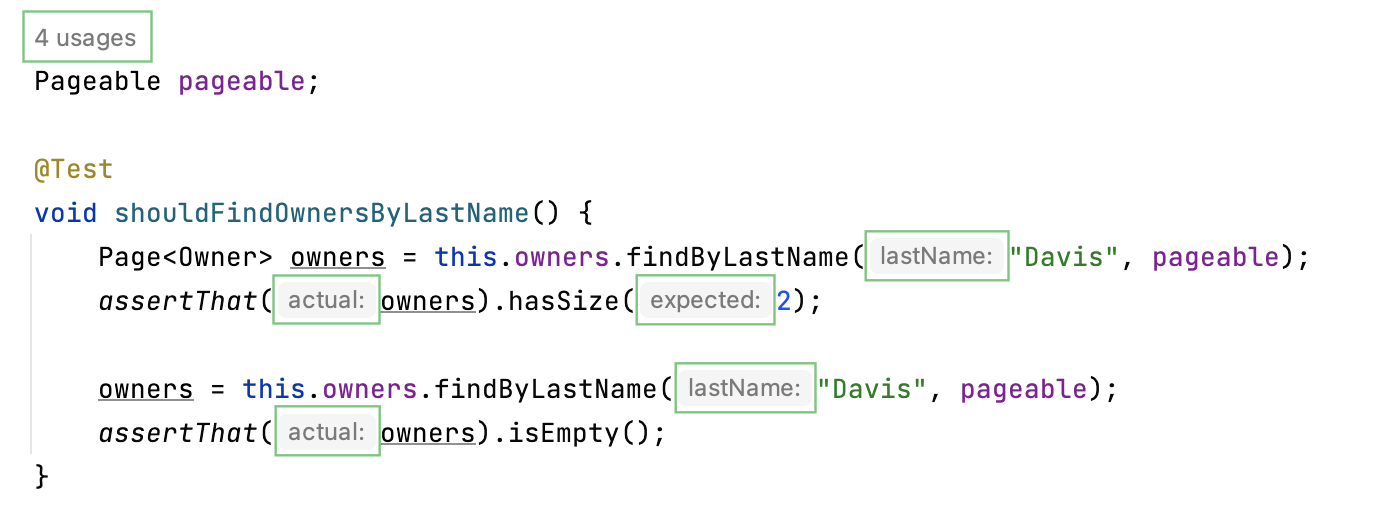
\includegraphics[width=0.95\textwidth]{figures/inlay_hints_example}
	\end{center}
	\caption{An example of inlay hints in the IntelliJ \gls{ide}. (From \web{https://www.jetbrains.com/help/idea/inlay-hints.html}{2024-10-04})}\label{fig:inlay}
\end{figure}


\section{Interim Conclusion}
In this chapter, we have taken a detailed look at the concepts behind the two topics central to this thesis---namely, the {Language Server Protocol} and \glspl{city}.
We have also motivated and laid out the specific ways in which the existing \gls{lsp} \glspl{capability} could be integrated into \SEE{}, including a formalization of the project graph that will become central to \cref{sec:generate}.

We are ready to tackle the actual implementation in the next chapter.
As a quick overview before then, \cref{tab:capabilities} lists the planned \glspl{capability} along with their intended use in \SEE{}.

\begin{table}[H]
	\caption{\gls{lsp} \glspl{capability} that will be integrated into \SEE{} as part of this thesis.}\label{tab:capabilities}
	\begin{tabularx}{\textwidth}{@{}lXX@{}}
		\toprule
		\multicolumn{1}{c}{\textbf{Capability}} & \multicolumn{1}{c}{\textbf{Code Windows}}                               & \multicolumn{1}{c}{\textbf{Code Cities}}            \\ \midrule
		\textit{Call hierarchy}                 & Show incoming/outgoing calls and allow jumping to caller                & Generate corresponding edges                        \\
		\textit{Diagnostics}                    & Highlight corresponding code \glspl{range} and display details on hover & Display code smell icons~\cite[see][]{galperin2021} \\
		\textit{References}                     & Show references and allow jumping to usage                              & Generate corresponding edges                        \\
		\textit{Document symbols}               & \multicolumn{1}{c}{---}                                                 & Generate corresponding nodes and hierarchy          \\
		\textit{Go to location$^*$}             & Show locations and allow jumping to them                                & Generate corresponding edges                        \\
		\textit{Hover}                          & Show hover information when hovering above item                         & Show hover information when hovering above node     \\
		\textit{\Glspl{token}}                  & Extended ("semantic") syntax highlighting                               & \multicolumn{1}{c}{---}                             \\
		\textit{Type hierarchy}                 & Show sub-/supertypes and allow jumping to them                          & Generate corresponding edges                        \\\bottomrule
	\end{tabularx}
	\caption*{\footnotesize $^*$This includes the \textit{Go to declaration / definition / implementation / type definition} capabilities.}
\end{table}

\end{document}
